% ----------------------------------------------------------------------
%  Pracovní úkoly
% ----------------------------------------------------------------------
\section{Pracovní úkoly}

\begin{enumerate}
\item Změřte závislost atmosférického tlaku na výšce.

\item Sestrojte graf závislosti tlaku na výšce a srovnejte s barometrickou rovnicí.

\end{enumerate}

% ----------------------------------------------------------------------
%  Teoretická část
% ----------------------------------------------------------------------
\section{Teoretická část}

Barometrická rovnice se používá pro popis změny atmosférického tlaku s nadmořskou výškou. Pro změnu tlaku $dp$ při změně výšky $dh$ s vrstvou vzduchu o hustotě $\rho$ a gravitačním zrychlením platí:

\begin{equation}
    dp = - \rho g dh
\end{equation}

Při proměnlivé hustotě vzduchu s výškou lze tuto závislost popsat tzv. Boyleova-Mariottova zákona. Po úpravě vztahu (1) dosazením vztahu pro hustotu a následnou integrací podle [3]

\begin{equation}
    \rho = \frac{\rho_0}{p_0}p
\end{equation}

kde $\rho_0$ a $p_0$ označuje nějakou známou hustotu a tlak. Dostáváme barometrickou rovnici

\begin{equation}
    p = p_0 \; e ^ {-\frac{\rho_0 g \Delta h}{p_0}}
\end{equation}

% ----------------------------------------------------------------------
%  Výsledky a zpracování měření
% ----------------------------------------------------------------------
\section{Výsledky a zpracování měření}

\subsection{Laboratorní podmínky}

V důsledku provádění experimentu uvnitř vysoké budovy City Tower na Pankráci v Praze, kde má sídlo Raiffensen bank je venkovní teplota irelevantní a uvnitř lze předpokládat přibližně pokojovou teplotu v každém patře po celou dobu měření, tedy přibližně 22 °C.

Měření bylo provedeno pomocí telefonu Apple iPhone 13, jehož barometr měří přibližně s nejistotou 1 hPa. Pro srovnání jsem zaznamenával také nadmořskou výšku vyhodnocenou na základě barometru hodinkami Garmin Epix pro.

\subsection{Výška pater budovy, nadmořská výška}
Nadmořská výška přízemí, tedy prostoru v okolí budovy, byla určena pomocí webové stránky mapy.cz jako

\begin{equation}
    \nonumber
    h_p = 268 \; m. n. m.
\end{equation}

Celková budova má 27 nadzemních a 3 podzemní podlaží. Měření bylo provedeno ve 28 patrech. Výška mezi jednotlivými patry je 4 metry. Poloha budovy je zobrazena na obrázku \ref{fig:city-tower-mapa}.

\begin{figure}[h]
    \centering
    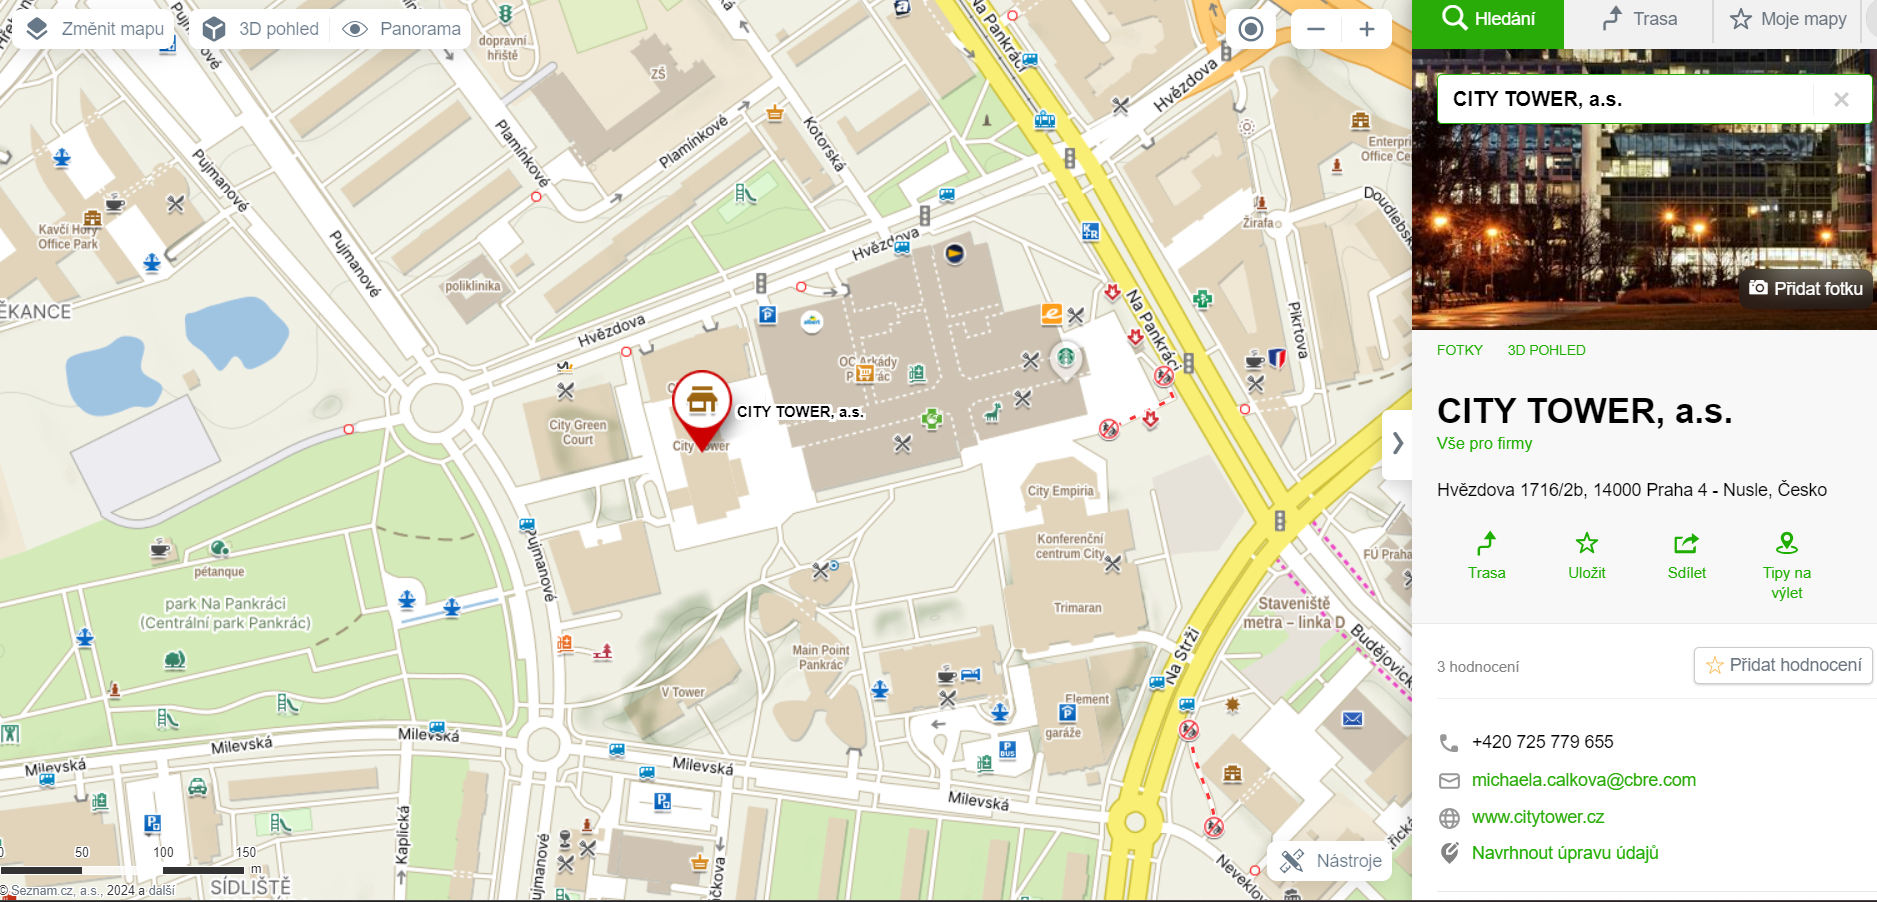
\includegraphics[width=1\linewidth]{Y1 - Závislost atmosférického tlaku na výšce – výletní//Protokol - závislost atmosférického tlaku na výšce – výletní//img/City Tower_mapy.png}
    \caption{Mapa City Tower}
    \label{fig:city-tower-mapa}
\end{figure}

\newpage

\subsection{Měření závislosti atmosférického tlaku na výšce}

Naměřené hodnoty jsou uvedeny v tabulce \ref{tab:namerene-hodnoty}. U každého patra je uvedena hodnota $\Delta h$, což je skutečná výška aktuálního patra od původního. Dále je uvedena výška, kterou udávají hodinky. Nakonec jsou uvedeny hodnoty $p_1$ a $p_2$ naměřených tlaků pří cestě vzhůru a poté dolů.

\begin{table}[h]
\centering
\caption{Naměřené hodnoty}
\label{tab:namerene-hodnoty}
\begin{tabular}{|c|c|c|c|c|}
\hline
Číslo patra & \Delta h / m & Výška podle hodinek / m & p_1 / Pa  & p_2 / Pa   \\ \hline
1           & 0       & 241           & 98788 & 98799 \\ \hline
2           & 4       & 245           & 98741 & 98751 \\ \hline
3           & 8       & 249           & 98702 & 98703 \\ \hline
4           & 12      & 253           & 98651 & 98649 \\ \hline
5           & 16      & 257           & 98620 & 98605 \\ \hline
6           & 20      & 261           & 98551 & 98568 \\ \hline
7           & 24      & 265           & 98500 & 98520 \\ \hline
8           & 28      & 269           & 98462 & 98470 \\ \hline
9           & 32      & 273           & 98411 & 98421 \\ \hline
10          & 36      & 277           & 98356 & 98369 \\ \hline
11          & 40      & 282           & 98310 & 98318 \\ \hline
12          & 44      & 286           & 98260 & 98265 \\ \hline
13          & 48      & 290           & 98220 & 98225 \\ \hline
14          & 52      & 294           & 98158 & 98167 \\ \hline
15          & 56      & 298           & 98116 & 9811  \\ \hline
16          & 60      & 302           & 98071 & 98088 \\ \hline
17          & 64      & 306           & 98031 & 98088 \\ \hline
18          & 68      & 310           & 97990 & 98003 \\ \hline
19          & 72      & 314           & 97952 & 97960 \\ \hline
20          & 76      & 318           & 97906 & 97976 \\ \hline
21          & 80      & 322           & 97868 & 97873 \\ \hline
22          & 84      & 326           & 97828 & 97828 \\ \hline
23          & 88      & 330           & 97782 & 97790 \\ \hline
24          & 92      & 334           & 97738 & 97744 \\ \hline
25          & 96      & 338           & 97702 & 97702 \\ \hline
26          & 100     & 342           & 97661 & 97663 \\ \hline
27          & 104     & 346           & 97620 & 97616 \\ \hline
28          & 108     & 350           & 97550 & 97502 \\ \hline
\end{tabular}
\end{table}

\newpage

Abychom mohly ukázat teoretickou závislost je třeba určit konstanty například na začátku měření, tedy v přízemí. Hustota vzduchu je při těchto podmínkách $\rho_0 = 1,157 \; kg/m^3$. Hodnota $p_0 = 98 788 \; Pa$.

Na obrázku \ref{fig:tlak-na-vysce} je zobrazena závislost atmosférického tlaku na nadmořské výšce. Jsou zde uvedeny hodnoty $p_1$, $p_2$ a $p_t$, která popisuje teoretickou nadmořskou výšku získanou z rovnice (3) dosazením konstant naměřených na počátku měření uvedených výše. Dále jsme naši naměřenou závislost fitovali exponenciální křivkou podle vztahu $p = A \; e^{R_0 \Delta h}$. Dostáváme $A = 5,8(7) \; kPa$ a $R_0 = -0,0022(3)$.

\begin{figure}[h]
    \centering
    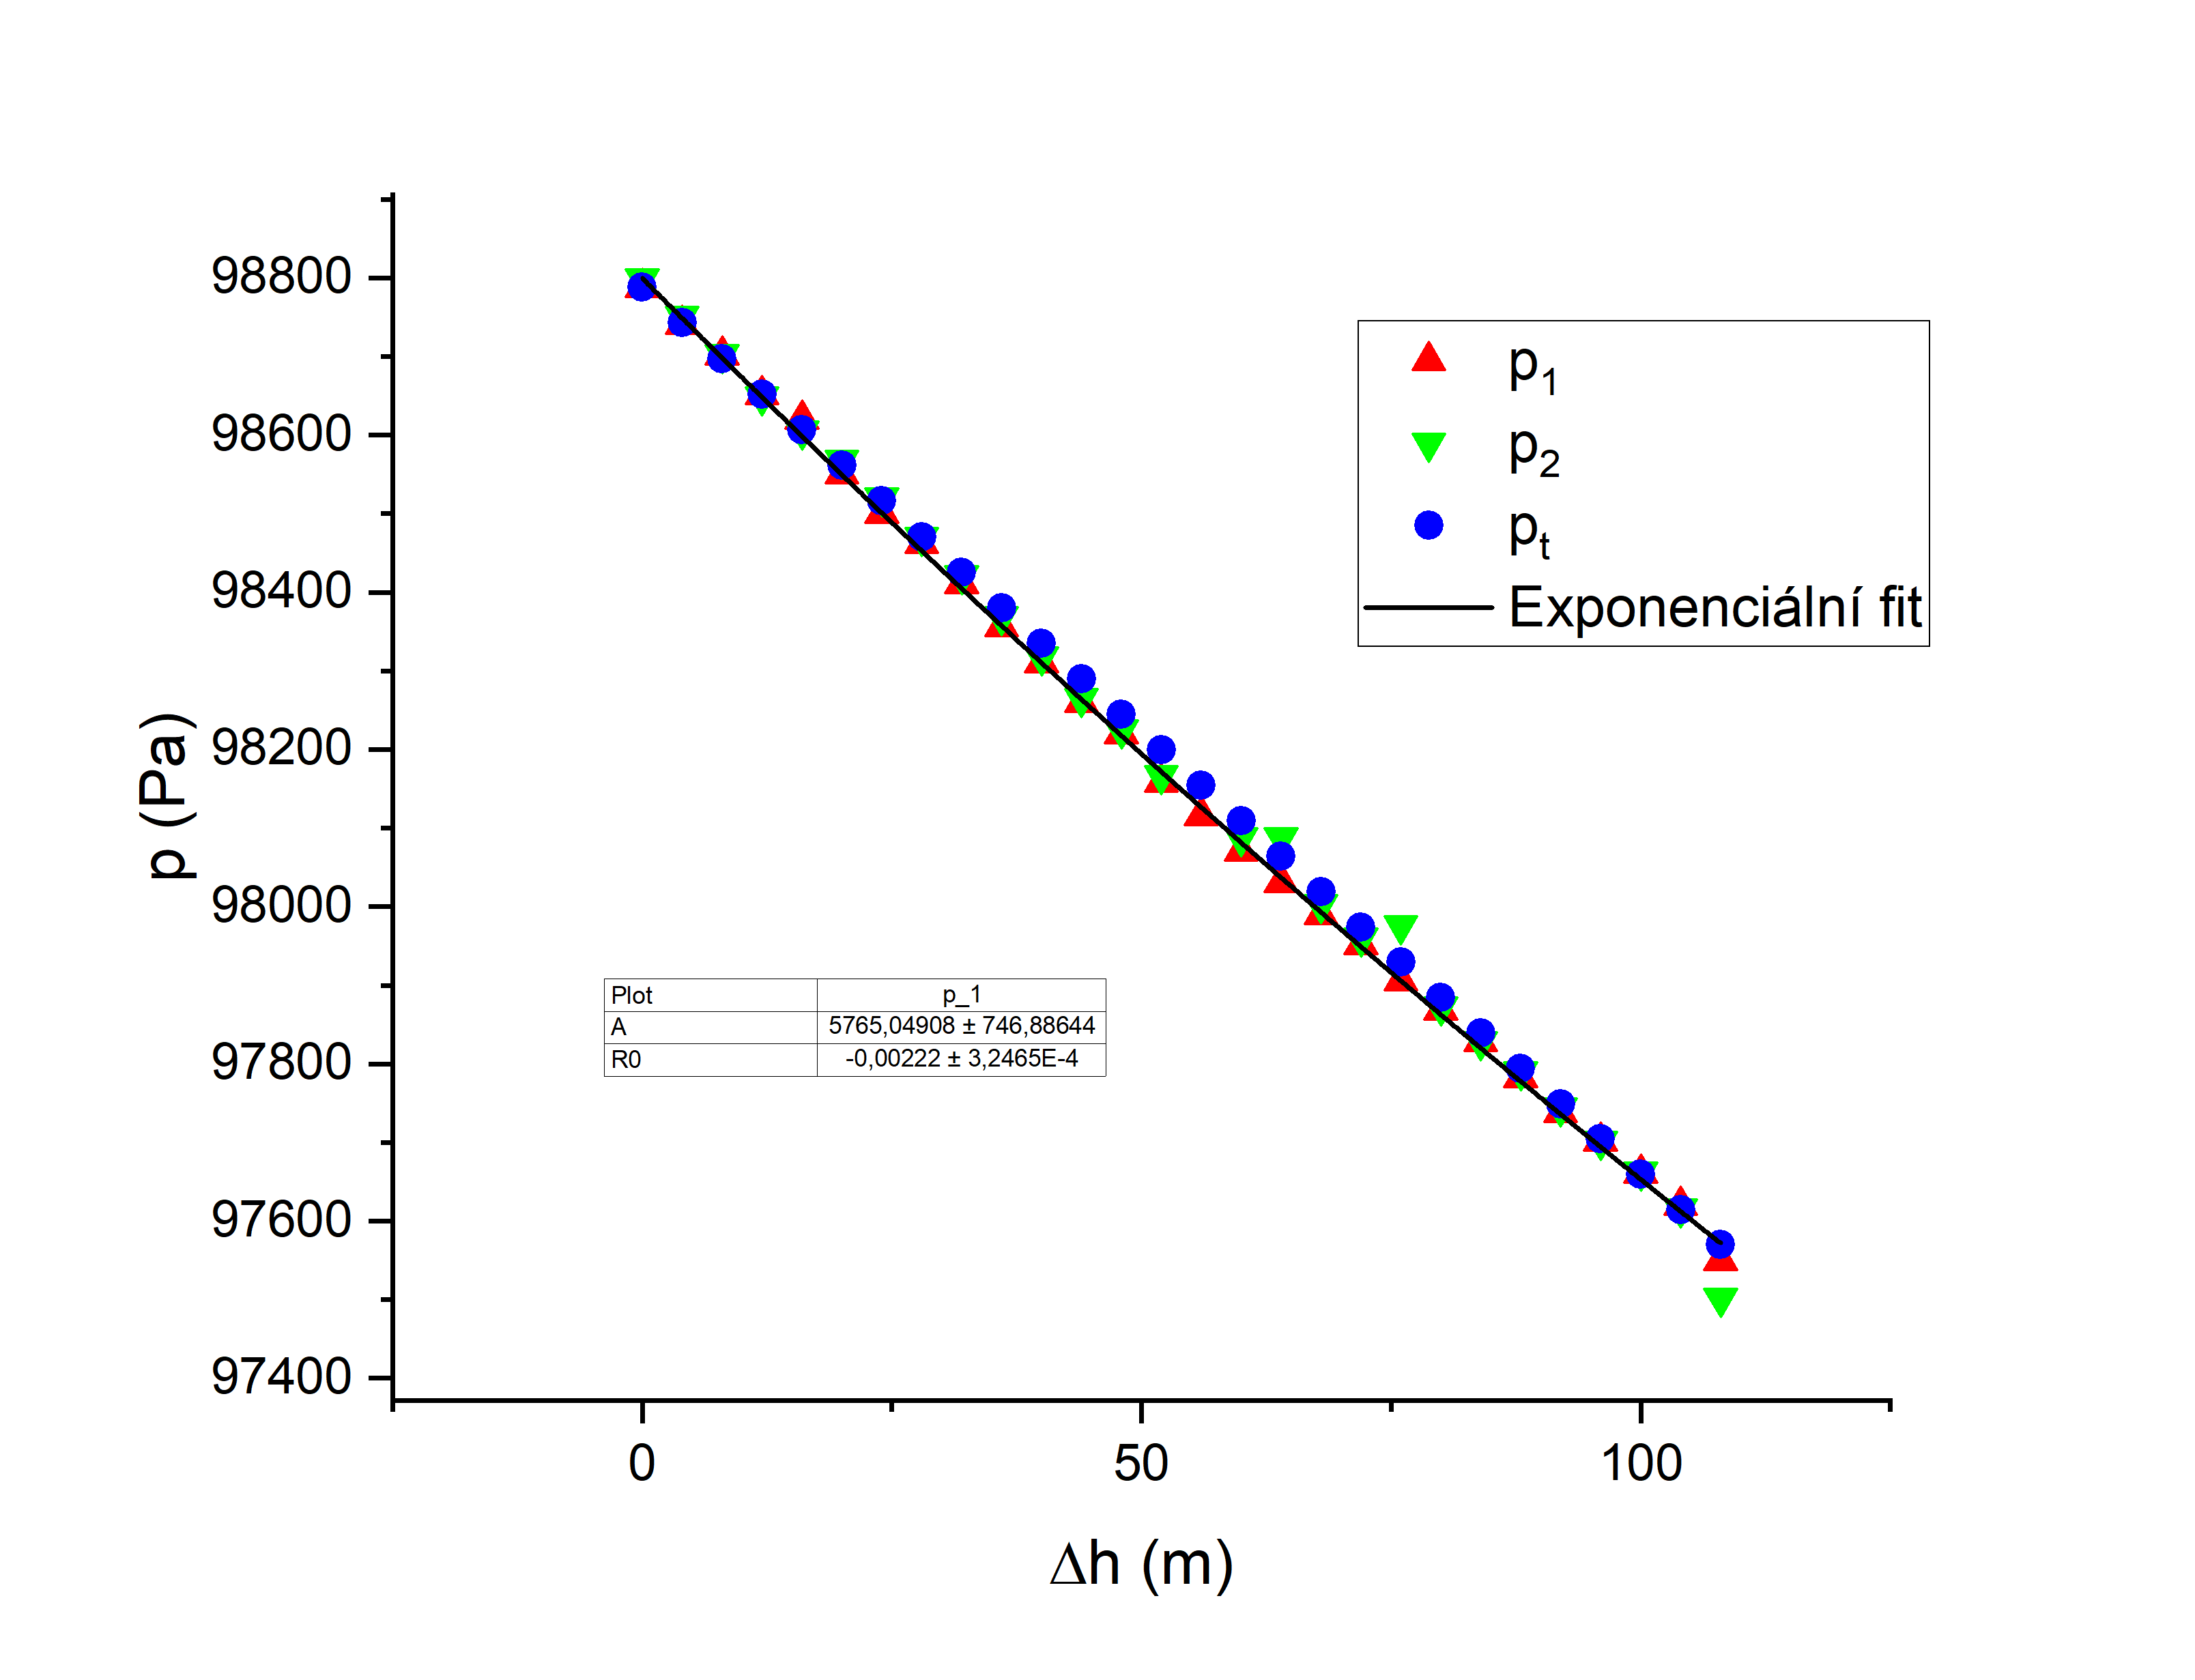
\includegraphics[width=1\linewidth]{Y1 - Závislost atmosférického tlaku na výšce – výletní//Protokol - závislost atmosférického tlaku na výšce – výletní//img/Závislost tlaku na výšce.png}
    \caption{Závislost atmosférického tlaku na nadmořské výšce}
    \label{fig:tlak-na-vysce}
\end{figure}

\newpage
% ----------------------------------------------------------------------
%  Diskuse výsledků
% ----------------------------------------------------------------------			
\section{Diskuse výsledků}

Naměřené hodnoty obou měření ($p_1$ a $p_2$) se shodují s předpokládanou teoretickou hodnotou. Naměřené hodnoty pomocí hodinek velmi přesně odpovídají výškovému rozdílu pater, avšak jsou všechny hodnoty posunuté o 27 m. n. m. To pravděpodobně znamená, že nebyly přesně kalibrovány, ale samotný barometr hodinek měří spolehlivě přesně. Lze odvozovat, že tato metoda měření je přesná a dobře popisuje realitu.

Samotná přesnost barometru telefonu je 1 hPa, která ve srovnaní s okolnostmi neovlivňuje výsledek a my ji tak můžeme zanedbat.

Mezi tyto okolnosti se řadí uvažování rovnice pro ideální laboratorní podmínky, které se mohou lišit od skutečnosti. Změna teploty s výškou by mohla mít vliv na měření, my jsme ale předpokládali konstantní teploty v celé budově. Protože jsme měřili na uzavřeném únikovém schodišti hodnoty tlaku mohly ovlivnit jednotlivé vrstvy budovy.

Naši závislost jsme fitovali exponenciální funkcí, jejíž hodnota koeficientu A vyšla přibližně 20x menší, než bychom mohli očekávat. Zdá se, že jsou špatně nastavené parametry fitu, ale to bylo několikrát zkontrolováno a provedeno znovu. Koeficient $R_0$ vychází dle očekávání. Lze předpokládat, že je výškový rozdíl natolik malý, že se daná závislost neprojeví. Na druhou stranu teoretická závislost se shoduje s naměřenými hodnotami, tak by měl být i fit podobný.

% ----------------------------------------------------------------------
%  Závěr
% ----------------------------------------------------------------------
\newpage

\begin{figure}
    \centering
    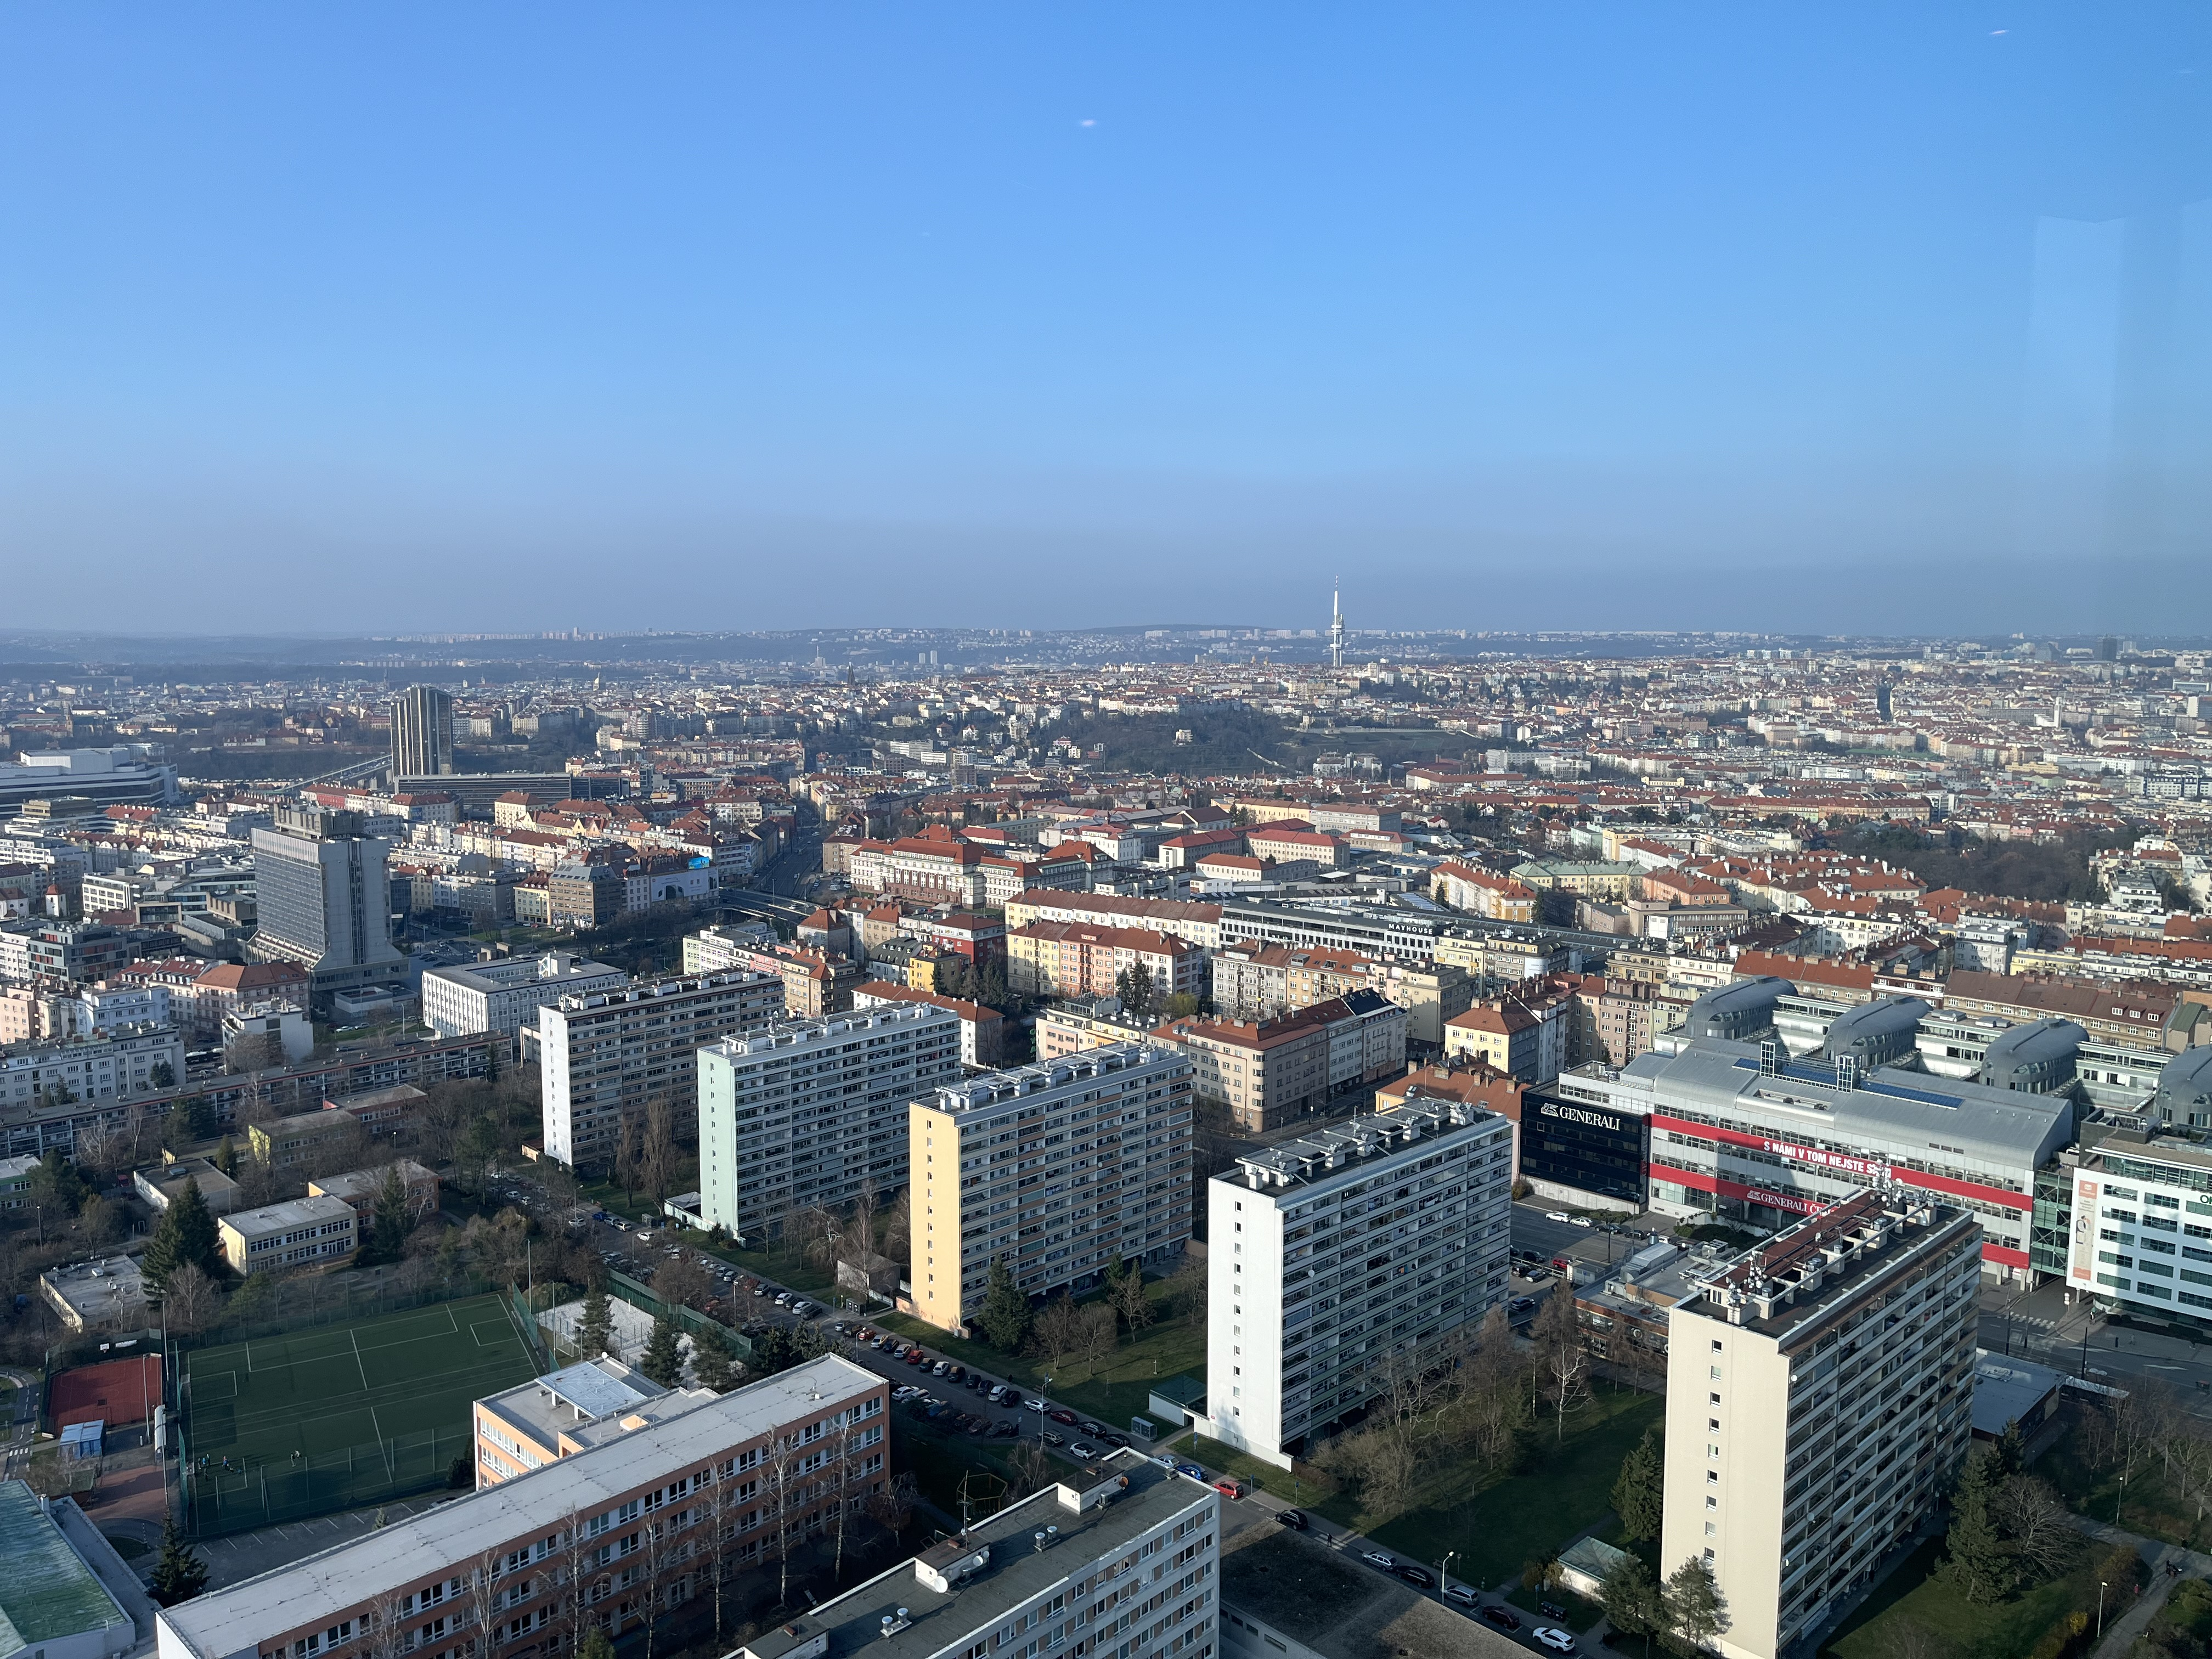
\includegraphics[width=0.75\linewidth]{Y1 - Závislost atmosférického tlaku na výšce – výletní//Protokol - závislost atmosférického tlaku na výšce – výletní//img/IMG_4358.jpg}
    \caption{Výhled z nejvyššího patra}
    \label{fig:vyhled}
\end{figure}

\section{Závěr}

V této práci jsme změřili závislost atmosférického tlaku na výšce. Dále jsme sestrojili graf této závislosti a porovnali jsme ho s barometrickou rovnicí. Naměřené hodnoty jsme fitovali exponenciální funkcí s koeficienty $A = 5,8(7) \; kPa$ a $R_0 = -0,0022(3)$. Navíc jsme zároveň provedli srovnávací měření druhým barometrem, kde jsme potvrdili přesnost s pravděpodobně ne úplně přesnou kalibrací zařízení na začátku měření.